\section{Experiments}
\label{sec:experiments}
\paragraph{Setup.}
We provide empirical support for each claim of \S\ref{sec:grpo}--\S\ref{sec:method} through a corresponding table or figure; unless noted otherwise, diagnostics use Game24, where the variants differ most (details: Appendix~\ref{app:results}; related work: Appendix~\ref{app:related}). Four program-verified tasks are evaluated: \textbf{Countdown}, \textbf{Sudoku}, \textbf{Knights-and-Knaves} (K\&K) and \textbf{Game24} (Appendix~\ref{app:datasets}). All runs start from ELF-B (105M) fine-tuned separately on each task, the base. Accuracy is measured on 2{,}000 held-out prompts (1{,}601 for Game24) under the deployment chain $\gamma56$@64 (churn $\gamma{=}56$, $K{=}64$ steps; $\gamma28$@32 on Sudoku) and the cheap chain $\gamma4$@16 ($\gamma14$@16 on Sudoku) through the same denoiser. \methodGRPO{} trains with the 16-step chain $\gamma4$@16, the SVG variants (Algorithm~\ref{alg:jpc}) with the deployment chain. GPT-2 \citep{radford2019gpt2} and LLaDA-8B-Instruct \citep{nie2025llada} with d1's recipe \citep{zhao2025d1}, trained on the same data, serve as cross-architecture references. We report peak held-out RL accuracy; Appendix~\ref{app:details} gives budgets and per-seed values.

\begin{table}[t]
\centering\small
\begin{minipage}[c]{0.615\linewidth}
\centering\footnotesize
\setlength{\tabcolsep}{1.5pt}
\begin{tabular}{@{}lcccc@{}}
\toprule
 & Countdown & Sudoku & K\&K & Game24 \\
\midrule
\multicolumn{5}{@{}l}{\emph{GPT-2 (124M, autoregressive)}}\\
task SFT & 44.2 & \phantom{0}1.2 & 92.9 & 26.9 \\
+ token GRPO/PPO & 61.8 {\scriptsize(+17.6)} & \phantom{0}1.4 {\scriptsize(+0.2)} & 93.3 {\scriptsize(+0.4)} & 46.6 {\scriptsize(+19.7)} \\
\midrule
\multicolumn{5}{@{}l}{\emph{LLaDA-8B-Instruct (masked diffusion)}}\\
task SFT & 13.1 & \phantom{0}0.7 & 61.0 & 16.1 \\
+ diffu-GRPO & 14.9 {\scriptsize(+1.8)} & \phantom{0}0.7 {\scriptsize(+0.0)} & 62.5 {\scriptsize(+1.5)} & 19.5 {\scriptsize(+3.4)} \\
\midrule
\multicolumn{5}{@{}l}{\emph{ELF-B (105M, continuous flow)}}\\
task SFT (base) & 42.2 & 66.2 & 67.5 & 45.0 \\
+ \methodGRPO{} & 43.1 {\scriptsize(+0.9)} & 69.7 {\scriptsize(+3.5)} & 71.6 {\scriptsize(+4.1)} & 47.5 {\scriptsize(+2.5)} \\
+ \methodSVGScalar{} & 48.2 {\scriptsize(+6.0)} & 66.3 {\scriptsize(+0.1)} & 77.6 {\scriptsize(+10.1)} & 51.4 {\scriptsize(+6.4)} \\
+ \hl{\methodSVGTwoD{}} & \textbf{50.2} {\scriptsize(+8.0)} & \textbf{71.0} {\scriptsize(+4.8)} & \textbf{79.6} {\scriptsize(+12.1)} & \textbf{58.8} {\scriptsize(+13.8)} \\
\bottomrule
\end{tabular}
\end{minipage}\hfill
\begin{minipage}[c]{0.37\linewidth}
\centering
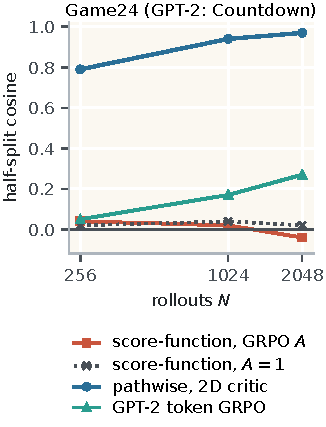
\includegraphics[width=\linewidth]{figures/fig_estimator.pdf}
\end{minipage}
\caption{\textbf{Left:} held-out accuracy (\%) under the deployment chain at the best checkpoint; RL rows carry the gain over their model's task-SFT row in parentheses; RL rows of GPT-2 and ELF\mbox{-}B are means of three seeds (Appendix~\ref{app:seeds}), LLaDA rows single runs; bold: best ELF\mbox{-}B row; blue: recommended variant. \textbf{Right:} Game24 rollouts of each model's SFT base; control: $A{=}1$ (top), a random direction (bottom) (Appendices~\ref{app:snr}, \ref{app:onestep}). Top: half-split cosine against the number of rollouts $N$. Bottom: accuracy change after one AdamW-normalised step, in units of $\Lambda$, the distance the 2D-critic run travels from the base; bands: paired $95\%$ intervals.}
\label{tab:main}
\end{table}

\paragraph{Main result.}\label{sec:exp_main}
Read Table~\ref{tab:main} down the ELF-B block, then across models. On the flow model the estimator decides the gain: \methodGRPO{} moves every task by a few points at most, \methodSVGScalar{} gains at least twice as much on three tasks (Sudoku excepted), and \methodSVGTwoD{}, which differs from it only in the critic, adds to that on every task. The cap is not intrinsic to the score-function estimator: GPT-2's token-level GRPO/PPO gains roughly ten times as much as \methodGRPO{} on Countdown and Game24, the two tasks where its supervised model is neither saturated nor near zero, while LLaDA's masked-diffusion surrogate gains a few points at most (further comparisons: Appendices~\ref{app:ar_curves}, \ref{app:grpo_variants}, \ref{app:d1}).

\paragraph{Why the score-function variant is capped.}\label{sec:exp_estimator}
Finer advantages, a second update per batch or the deployment chain move \methodGRPO{} by a few points on some tasks, none closes the gap to \methodSVGTwoD{}, and restoring the KL anchor ($\beta>0$) removes even those points (Appendices~\ref{app:sf_variants}, \ref{app:grpo_variants}, \ref{app:grpo_chain}). Tuning the recipe is therefore unlikely to be the limitation; \S\ref{sec:grpo} points to the action space, one reward bit supervising $(K-2)\,|\mathcal G|\,d$ noise coordinates per rollout. The right panels of Table~\ref{tab:main} test this on Game24 rollouts of the base (Countdown: Appendix~\ref{app:onestep}; discrete baselines: Appendix~\ref{app:discrete_snr}). \emph{Top:} we split $N$ rollouts in half and measure the cosine between the two mean gradients; a genuine signal drives it towards one as $N$ grows, pure noise leaves it near zero. \methodGRPO{}'s gradient stays indistinguishable from the $A{=}1$ control (every advantage set to one, a gradient of mean zero) at every $N$; GPT-2's token-level gradient separates from the control as $N$ grows; the pathwise gradient through the critic agrees across halves from the smallest $N$. Agreement is not correctness. \emph{Bottom:} we step once from the base along each mean gradient, AdamW-normalised, and re-evaluate, which tests the direction. At a quarter and a half of $\Lambda$ the pathwise step improves accuracy with intervals that exclude zero, whereas the score-function step gains under two points with intervals that include zero; at a full $\Lambda$ the pathwise gain turns over, consistent with a critic that is not refit being followed too far. Without AdamW's per-coordinate normalisation the same pathwise gradient destroys the policy, its norm being concentrated in a few coordinates (Appendix~\ref{app:onestep}).

\begin{table}[!b]
\centering\small
\begin{minipage}[c]{0.60\linewidth}
\centering
\setlength{\tabcolsep}{3pt}
\resizebox{\linewidth}{!}{%
\begin{tabular}{@{}lcccc@{}}
\toprule
critic & Pearson & pick@$V_\phi$ & best & final \\
\midrule
fine-tuned copy, reads $(y_k,\hat x_{k-1})$ & \CDa{1} & \CDa{3} & \CDa{5} & \CDa{6} \\
\quad without $\hat x_{k-1}$ in the input & \CDb{1} & \CDb{3} & \CDb{5} & \CDb{6} \\
\quad copy frozen in pre-training & \CDc{1} & \CDc{3} & \CDc{5} & \CDc{6} \\
\quad random initialisation & \CDd{1} & \CDd{3} & 37.9 & \phantom{0}4.1 \\
\quad copy also trained in RL & \CDa{1} & \CDa{3} & 49.7 & 49.3 \\
\quad frozen in RL$^\dagger$ & --- & --- & 48.4 & \phantom{0}0.3 \\
\bottomrule
\end{tabular}}
\end{minipage}\hfill
\begin{minipage}[c]{0.385\linewidth}
\centering
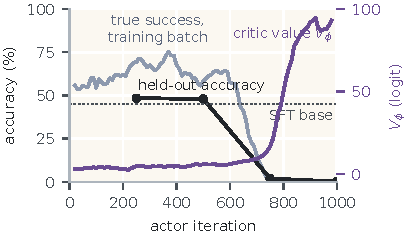
\includegraphics[width=\linewidth]{figures/fig_frozen.pdf}
\end{minipage}
\caption{\textbf{Left:} the 2D critic of Algorithm~\ref{alg:jpc} on Game24 (first row) and variants with one element changed. \emph{Offline}, on held-out base rollouts at step 32 of 64: Pearson correlation of the pooled value with the outcome, and pick@$V_\phi$, the success rate of the top-ranked of eight rollouts (chance $0.55$). \emph{Online}: held-out accuracy (\%) of one RL run at its best and final checkpoint (---: not measured). \textbf{Right:} the frozen-critic run over training ($^\dagger$earlier recipe, Appendix~\ref{app:details}); the critic's value is on the right axis, in logits.}
\label{tab:critic_design}
\end{table}

\paragraph{What the critic must be.}\label{sec:exp_critic}
Table~\ref{tab:critic_design} evaluates the critic of Algorithm~\ref{alg:jpc} and its variants offline and in policy training. Removing $\hat x_{k-1}$ from the input or freezing the copy during pre-training lowers the offline correlation by about a third or more, and the policy improves briefly before collapsing. A randomly initialised network never clears the base: the estimate carries the outcome information, and the pre-trained denoiser is what reads it (\S\ref{sec:critic}); training the copy along with the head during RL also falls short (Appendix~\ref{app:critic_training}). The last row, plotted over training in the right panel, shows that the critic must also track the policy: frozen after pre-training it is exploited, as the bias~(\ref{eq:biasm}) leads one to expect, its value on the training batch driven to certainty while the batch's true success collapses. Refitting the head prevents this (\S\ref{sec:joint}).

\begin{figure}[t]
\centering
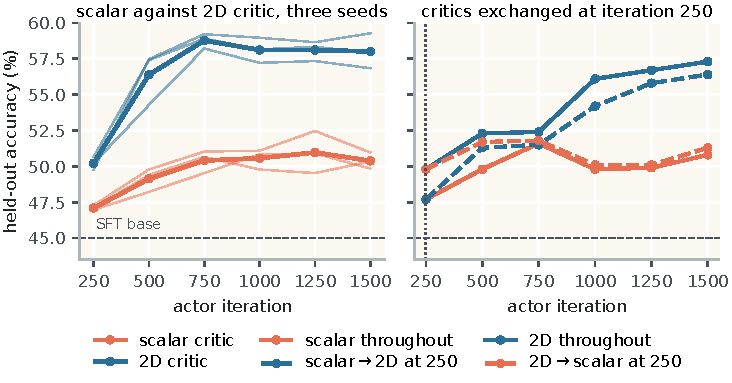
\includegraphics[width=0.85\linewidth]{figures/fig_dyn.pdf}
\caption{Game24, held-out accuracy (\%) under the deployment chain. \textbf{Left:} the scalar- and 2D-critic runs of Table~\ref{tab:main}, three seeds (thin) and their mean (thick). \textbf{Right:} critics exchanged at iteration 250 between a fourth seed of each run (2D head refit with the first term of~(\ref{eq:critic2d_loss}) only, equivalent on Game24); the colour marks the critic in charge after the exchange (values: Appendix~\ref{app:swap_late}).}
\label{fig:dyn}
\end{figure}

\paragraph{The 2D critic keeps the update improving.}\label{sec:exp_2d}
Figure~\ref{fig:dyn} (left) tracks held-out accuracy for the scalar- and 2D-critic runs of Table~\ref{tab:main}. The scalar critic's policy flattens after about 500 iterations while the 2D critic's continues to improve and holds its gain (other tasks: Appendix~\ref{app:traj}). On states sampled from one policy, however, the two critics perform similarly (Appendix~\ref{app:critic_equiv}). The right panel locates the difference by exchanging the critics at iteration 250, while the two policies are still within a few points: each run ends where the critic in charge thereafter takes it, and exchanging after the policy has flattened changes little (Appendix~\ref{app:swap_late}). The 2D critic therefore produces its advantage as the policy evolves.

Two elements of \S\ref{sec:jpc_2d} could carry this: the head applied per position, so that each reading shapes the actor through its own slope~(\ref{eq:headgrad}), and the per-position loss term of~(\ref{eq:critic2d_loss}). Both critics are exploited when frozen, so the advantage can only arise under the refit (Appendices~\ref{app:critic_equiv}, \ref{app:frozen}). On Game24, refitting the head-before-mean critic with the pooled loss alone is sufficient; on Countdown, where the scalar critic loses discrimination as its policy turns, the per-position loss is also necessary (Appendix~\ref{app:needs_full}).

\paragraph{Ablations.}\label{sec:ablations}
Table~\ref{tab:needs} reports ablations of the stated design choices on Game24 (the rest: Appendix~\ref{app:needs_full}). Log-odds beats probability as the objective (\S\ref{sec:pathwise}), and the mean beats the minimum as the pooling (\S\ref{sec:jpc_2d}; why the minimum serves search instead: Appendix~\ref{app:loop}). A decaying step size keeps the seeds near their peaks, whereas a constant rate declines and a larger one collapses, as the step-proportional bias of \S\ref{sec:joint} predicts (Appendix~\ref{app:lr_regime}); refitting only at the window's last step is neutral on Game24 (not in Table~\ref{tab:needs}; Appendix~\ref{app:needs_full}). The last row motivates the amortisation loop: a run trained under the cheap chain gains there but carries little of it to the deployment chain (Appendix~\ref{app:needs_full}; Table~\ref{tab:loop}).

\begin{table}[!t]
\centering\small
\caption{Ablations of Algorithm~\ref{alg:jpc} on Game24: held-out accuracy (\%) under the deployment chain at the best and the last checkpoint. Variants are single runs (seed spread about a point, Appendix~\ref{app:results_fig}); each reference is the three-seed mean of the unablated recipe its variant departs from (rows 1--2, 3--4 and 5: recipe blocks A, B and C of Appendix~\ref{app:details}; trajectories and the Countdown rows: Appendix~\ref{app:needs_full}).}
\label{tab:needs}
\setlength{\tabcolsep}{5pt}
\begin{tabular*}{\linewidth}{@{\extracolsep{\fill}}llcc@{}}
\toprule
choice it tests & variant & best / final & reference \\
\midrule
\S\ref{sec:pathwise}, objective & actor ascends $\mathrm{sig}(V_\phi)$ instead of $V_\phi$ & \ABp{7} / \ABp{6} & 58.8 / 58.0 \\
\S\ref{sec:jpc_2d}, pooling & actor ascends $\min_iR_{k,i}$ instead of the mean & \ABm{7} / \ABm{6} & 58.8 / 58.0 \\
\S\ref{sec:joint}, step size & learning rate $3\times10^{-6}$ & 58.0 / 30.3 & 58.9 / 58.4 \\
\S\ref{sec:joint}, step size & constant learning rate $10^{-6}$ & 57.9 / 48.7 & 58.9 / 58.4 \\
\S\ref{sec:joint}, one chain & trained under the cheap chain, read at deployment & 47.0 / 47.0 & 56.4 / 56.4 \\
\bottomrule
\end{tabular*}
\end{table}



\paragraph{The loop.}\label{sec:exp_loop}
Table~\ref{tab:loop} evaluates Algorithm~\ref{alg:loop} on the three tasks with a pool of unlabelled problems (pools and Game24: Appendices~\ref{app:details}, \ref{app:g24_loop}). On Countdown and K\&K, the loop raises the cheap chain to or beyond the base model's deployment accuracy, transferring the gains across chains. The loop is limited by both coverage and pool novelty (Proposition~\ref{prop:em}; Appendix~\ref{app:loop}): K\&K reaches near-perfect accuracy with broad coverage, from any start, whereas on Sudoku even full-coverage gold solutions add only about a point. On Countdown, plain rounds reduce coverage and partially erase the RL gain; rounds drawn with the critic-guided cheap chain restore both (chain and guidance change together; Appendix~\ref{app:loop_full}).

\begin{table}[H]
\centering\small
\caption{Held-out accuracy (\%) under the cheap and the deployment chain: the base, the 2D-critic policy the loop starts from (best seed), and the model after the rounds. Bold: over a point above the start; blue: recommended variant; covered: pool problems with a verified sample (all rounds and controls: Appendix~\ref{app:loop_full}).}
\label{tab:loop}
\begin{tabular*}{\linewidth}{@{\extracolsep{\fill}}lcccccc@{}}
\toprule
 & \multicolumn{2}{c}{Countdown (4 rounds)} & \multicolumn{2}{c}{K\&K (5 rounds)} & \multicolumn{2}{c}{Sudoku (1 round)} \\
\cmidrule{2-3}\cmidrule{4-5}\cmidrule{6-7}
 & cheap & deploy. & cheap & deploy. & cheap & deploy. \\
\midrule
base & 23.1 & 42.2 & 58.1 & 67.5 & 62.0 & 66.2 \\
2D-critic policy (loop start) & 23.9 & 50.4 & 68.8 & 80.0 & 65.0 & 71.3 \\
\hl{+ amortisation loop} & \textbf{\OURScdg} & 50.2 & \textbf{\OURSkkg} & \textbf{\OURSkk} & 65.5 & 71.4 \\
\midrule
pool covered by round (of 50k) & \multicolumn{2}{c}{35k, 31k, 37k, 38k} & \multicolumn{2}{c}{41k $\to$ 49k} & \multicolumn{2}{c}{39k} \\
\bottomrule
\end{tabular*}
\end{table}
